% Generated by code/needham.py -- do not edit by hand.
\definecolor{qocA}{rgb}{0.00,0.45,0.70}
\definecolor{qocB}{rgb}{0.90,0.60,0.00}
\definecolor{qocC}{rgb}{0.00,0.62,0.45}
\definecolor{qocD}{rgb}{0.80,0.40,0.00}
\definecolor{qocE}{rgb}{0.80,0.60,0.70}
\definecolor{qocF}{rgb}{0.35,0.70,0.90}
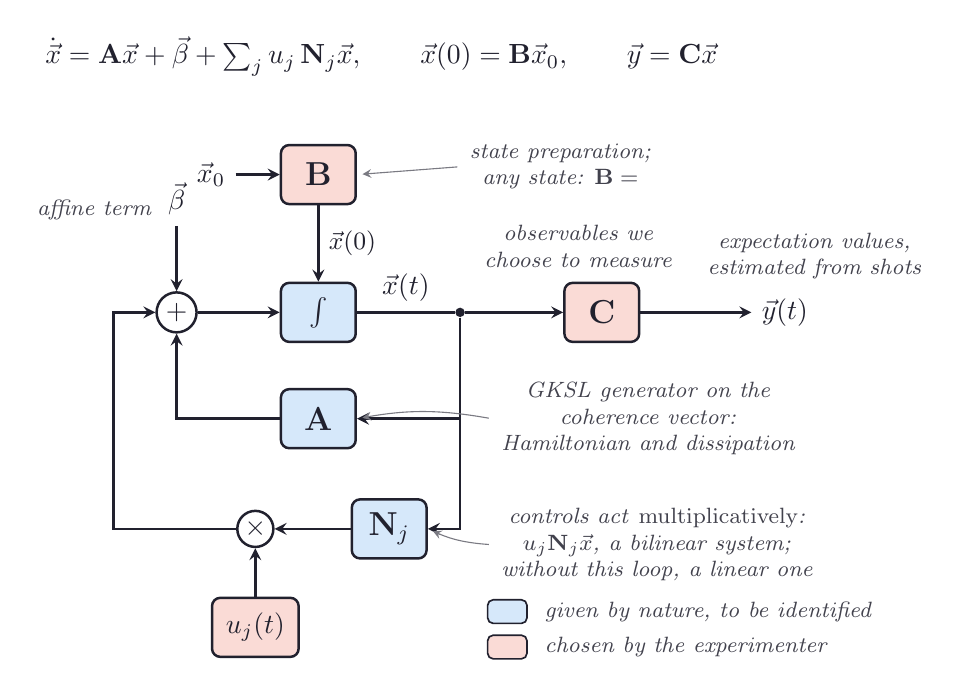
\begin{tikzpicture}[ink/.style={line width=0.9pt, ndInk}, faint/.style={line width=0.4pt, ndInk!35}, dashedink/.style={line width=0.5pt, ndInk!55, dash pattern=on 2.5pt off 2pt}, vec/.style={->, >=stealth, line width=1.2pt}, note/.style={font=\footnotesize\itshape, text=ndInk!85, align=center}, pointer/.style={->, >=stealth, line width=0.4pt, ndInk!60, shorten >=2pt, shorten <=1pt}, dot/.style={circle, fill=ndInk, inner sep=0pt, minimum size=3.4pt}, wash/.style={fill=ndSky, fill opacity=0.55}, every node/.style={text=ndInk}]
\definecolor{ndInk}{rgb}{0.13,0.13,0.18}
\definecolor{ndPaper}{rgb}{0.99,0.96,0.88}
\definecolor{ndSky}{rgb}{0.84,0.91,0.98}
\definecolor{ndRose}{rgb}{0.98,0.86,0.84}
\definecolor{ndBlue}{rgb}{0.13,0.36,0.66}
\definecolor{ndRed}{rgb}{0.78,0.20,0.16}
\definecolor{ndGold}{rgb}{0.88,0.62,0.10}
\definecolor{ndGreen}{rgb}{0.18,0.52,0.30}
\node at (5.6,3.25) {$\dot{\vec x}=\mathbf A\vec x+\vec\beta+\sum_j u_j\,\mathbf N_j\vec x,\qquad \vec x(0)=\mathbf B\vec x_0,\qquad \vec y=\mathbf C\vec x$};
\node[circle, draw=ndInk, line width=0.9pt, inner sep=1.5pt, fill=white] (S) at (3.0,0) {$+$};
\node[draw=ndInk, line width=0.9pt, rounded corners=3pt, minimum width=0.95cm, minimum height=0.75cm, font=\large, fill=ndSky] (I) at (4.8,0) {$\int$};
\node[dot] (P) at (6.6,0) {};
\node[draw=ndInk, line width=0.9pt, rounded corners=3pt, minimum width=0.95cm, minimum height=0.75cm, font=\large, fill=ndRose] (C) at (8.4,0) {$\mathbf C$};
\node[draw=ndInk, line width=0.9pt, rounded corners=3pt, minimum width=0.95cm, minimum height=0.75cm, font=\large, fill=ndRose] (B) at (4.8,1.75) {$\mathbf B$};
\node[draw=ndInk, line width=0.9pt, rounded corners=3pt, minimum width=0.95cm, minimum height=0.75cm, font=\large, fill=ndSky] (A) at (4.8,-1.35) {$\mathbf A$};
\node[draw=ndInk, line width=0.9pt, rounded corners=3pt, minimum width=0.95cm, minimum height=0.75cm, font=\large, fill=ndSky] (Nj) at (5.7,-2.75) {$\mathbf N_j$};
\node[circle, draw=ndInk, line width=0.9pt, inner sep=1pt, fill=white] (M) at (4.0,-2.75) {$\times$};
\node[draw=ndInk, line width=0.9pt, rounded corners=3pt, minimum width=0.95cm, minimum height=0.75cm, font=\large, fill=ndRose, minimum width=1.1cm, font=\normalsize] (U) at (4.0,-4.0) {$u_j(t)$};
\draw[->, >=stealth, line width=0.9pt, ndInk] (S) -- (I);
\draw[line width=0.9pt, ndInk] (I) -- node[above] {$\vec x(t)$} (P);
\draw[->, >=stealth, line width=0.9pt, ndInk] (P) -- (C);
\draw[->, >=stealth, line width=0.9pt, ndInk] (C) -- (10.3,0) node[right] {$\vec y(t)$};
\draw[->, >=stealth, line width=0.9pt, ndInk] (3.75,1.75) node[left] {$\vec x_0$} -- (B);
\draw[->, >=stealth, line width=0.9pt, ndInk] (B) -- node[right, font=\small] {$\vec x(0)$} (I);
\draw[->, >=stealth, line width=0.9pt, ndInk] (3.0,1.1) node[above] {$\vec\beta$} -- (S);
\draw[->, >=stealth, line width=0.9pt, ndInk] (P) |- (A);
\draw[->, >=stealth, line width=0.9pt, ndInk] (A) -| (S);
\draw[->, >=stealth, line width=0.9pt, ndInk] (P) |- (Nj);
\draw[->, >=stealth, line width=0.9pt, ndInk] (Nj) -- (M);
\draw[->, >=stealth, line width=0.9pt, ndInk] (U) -- (M);
\draw[->, >=stealth, line width=0.9pt, ndInk] (M) -| (2.2,0) -- (S);
\node[note, anchor=west] (nB) at (6.6,1.85) {state preparation;\\ any state: $\mathbf B=\Id$};
\draw[pointer] (nB.west) -- (B.east);
\node[note, anchor=south] at (8.1,0.45) {observables we\\ choose to measure};
\node[note, anchor=south] at (11.1,0.3) {expectation values,\\ estimated from shots};
\node[note, anchor=west] (nA) at (7.0,-1.35) {GKSL generator on the\\ coherence vector:\\ Hamiltonian and dissipation};
\draw[pointer] (nA.west) to[bend right=10] (A.east);
\node[note, anchor=west] (nN) at (7.0,-2.95) {controls act \emph{multiplicatively}:\\ $u_j\mathbf N_j\vec x$, a bilinear system;\\ without this loop, a linear one};
\draw[pointer] (nN.west) to[bend left=10] (Nj.east);
\node[note, anchor=east] at (2.8,1.3) {affine term};
\node[draw=ndInk, line width=0.6pt, rounded corners=2pt, fill=ndRose, minimum width=0.5cm, minimum height=0.3cm] at (7.2,-4.25) {};
\node[note, anchor=west] at (7.55,-4.25) {chosen by the experimenter};
\node[draw=ndInk, line width=0.6pt, rounded corners=2pt, fill=ndSky, minimum width=0.5cm, minimum height=0.3cm] at (7.2,-3.8) {};
\node[note, anchor=west] at (7.55,-3.8) {given by nature, to be identified};
\end{tikzpicture}
